\documentclass{sig-alternate}%[conference][letterpaper]
\usepackage{times,amsmath}
\usepackage{epsfig,algorithm,caption,subcaption,multirow,multicol}
\usepackage[noend]{algpseudocode}
\usepackage[normalem]{ulem}
%\usepackage{color,url}
\usepackage{balance}

\usepackage{listings} % Required for inserting code snippets
\usepackage[usenames,dvipsnames]{color} % Required for specifying custom colors and referring to colors by name
\usepackage{url}
\definecolor{DarkGreen}{rgb}{0.0,0.4,0.0} % Comment color
\definecolor{highlight}{RGB}{255,251,244} % Code highlight color

\DeclareCaptionType{copyrightbox}

\newcommand{\secref}[1]{Section \ref{#1}}
\newcommand{\figref}[1]{Figure \ref{#1}}
\newcommand{\equref}[1]{Equation (\ref{#1})}
\newcommand{\exref}[1]{Example \ref{#1}}

\newcommand{\KZ}[1]{\textcolor{green}{[KZ: #1]}}
\newcommand{\JK}[1]{\textcolor{blue}{[JK: #1]}}
\newcommand{\myurl}[1]{\textsf{{\uline{#1}}}}

\newcommand{\cut}[1]{}
\newcommand{\myskip}{\vspace*{1ex}}
\newcommand{\shrink}{\vspace*{-1ex}}

%\theoremstyle{definition}
%\newenvironment{example}[1][Ex.]{\begin{trivlist}
%\item[\hskip \labelsep {\bfseries #1}]}{\end{trivlist}}
\newtheorem{example}{Example}
\newtheorem{theorem}{Theorem}[section]
\newtheorem{Problem}[theorem]{Problem}

\newcommand{\lbb}{{\color{black} \textbf{[}}}
\newcommand{\rbb}{{\color{black} \textbf{]}}}
\newcommand{\N}{\mathcal{C}}
\newcommand{\lb}{\mathcal{L}}
%
%%%%%%%%%%%%%%%%%%%%%%%%%%%%%%%%%%%%%%%%%%%%%%%%%%%%%%%%%%%%%%%%%%%%%%%%%%%
\lstdefinestyle{Style1}{ % Define a style for your code snippet, 
%multiple definitions can be made if, for example, you wish to insert 
%multiple code snippets using different programming languages into one document
language=c, % Detects keywords, comments, strings, functions, etc for the language specified
backgroundcolor=\color{highlight}, % Set the background color for the snippet - useful for highlighting
basicstyle=\footnotesize\ttfamily, % The default font size and style of the code
breakatwhitespace=false, % If true, only allows line breaks at white space
breaklines=true, % Automatic line breaking (prevents code from protruding outside the box)
captionpos=b, % Sets the caption position: b for bottom; t for top
commentstyle=\usefont{T1}{pcr}{m}{sl}\color{DarkGreen}, % Style of comments within the code - dark green courier font
deletekeywords={}, % If you want to delete any keywords from the current language separate them by commas
%escapeinside={\%}, % This allows you to escape to LaTeX using the character in the bracket
%firstnumber=1, % Line numbers begin at line 1
frame=single, % Frame around the code box, value can be: none, leftline, topline, bottomline, lines, single, shadowbox
frameround=tttt, % Rounds the corners of the frame for the top left, top right, bottom left and bottom right positions
keywordstyle=\color{Blue}\bf, % Functions are bold and blue
morekeywords={}, % Add any functions no included by default here separated by commas
rulecolor=\color{black}, % Frame border color
showstringspaces=false, % Don't put marks in string spaces
showtabs=false, % Display tabs in the code as lines
%stepnumber=5, % The step distance between line numbers, i.e. how often will lines be numbered
stringstyle=\color{Purple}, % Strings are purple
tabsize=2, % Number of spaces per tab in the code
}

% Create a command to cleanly insert a snippet with the style above anywhere in the document
\newcommand{\insertcode}[2]{\begin{itemize}\item[]\lstinputlisting[caption=#2,label=#1,style=Style1]{#1}\end{itemize}} % The first argument is the script location/filename and the second is a caption for the listing
%%%%%%%%%%%%%%%%%%%%%%%%%%%%%%%%%%%%%%%%%%%%%%%%%%%%%%%%%%%%%%%%%%%%%%%%%%%%%%%%%%
%
\newfont{\mycrnotice}{ptmr8t at 7pt}
\newfont{\myconfname}{ptmri8t at 7pt}
\let\crnotice\mycrnotice
\let\confname\myconfname

\begin{document}
\title{Probabilistic Code Topic Mining with Hierarchical Taxonomy}

\numberofauthors{3}
\author{%
\alignauthor
Kai Jiang\\
	\affaddr{Shanghai Jiao Tong University}\\
	\affaddr{Shanghai, China}\\
    \affaddr{jkai@sjtu.edu.cn}
\alignauthor
Yuanfei Zhu\\
	\affaddr{Shanghai Jiao Tong University}\\
	\affaddr{Shanghai, China}\\
	\affaddr{stanbird@sjtu.edu.cn}
\alignauthor
Kenny Q. Zhu\\
	\affaddr{Shanghai Jiao Tong University}\\
	\affaddr{Shanghai, China}\\
    \affaddr{kzhu@cs.sjtu.edu.cn}
}
\maketitle

\begin{abstract}

\end{abstract}

% NOTE keywords are not used for conference papers so do not populate them
\begin{keywords}
Probabilistic graphical model; Source code mining; Taxonomy
\end{keywords}
\setlength{\floatsep}{2.2mm plus 1mm minus 1mm}
\setlength{\textfloatsep}{2.2mm plus 1mm minus 1mm}
\setlength{\intextsep}{2.2mm plus 1mm minus 1mm}
\section{Introduction}

Protein$-$protein interactions (PPIs) are of central importance for the majority of biological functions, such as signal transduction, metabolic pathways, molecular dynamics, and protein networks\cite{Hoffmann.Krallinger.ea:2005}, for they serve as the most fundamental building blocks of the entire interacademic systems of any organisms. Collecting data on pairwise interaction relationships is essential for multiple purpose, including identification of modules with certain functionality\cite{Spirin.Mirny.03}, mapping diseases to dominated genes\cite{Ideker.Sharan.08}, and after all, understanding wholistic metabolic/genetic networks from a system biology perspective.

A lot of databases have been built to store protein and genetic interactions from major model organism species and are available in various standardized formats, such as MINT\cite{Zanzoni.Montecchi-Palazzi.ea:2002}, BIND\cite{Bader.ea:2003}, BIOGRID\cite{DBLP:journals/nar/StarkBRBBT06}, etc. Among those mainstream databases, the data largely rely on voluntary reports by scientists or researchers, besides, comprehensive curation efforts become indispensable for the sake of accuracy. However, the amount of biology-related literatures with respect to protein interactions grows explosively and thus make it either impossible or impractical to manually detect PPI information anymore.

Considering huge amount of PPI information with great wealth hidden in published papers, in recent years, numerous mining techniques have been proposed that aim to extract PPI information automatically from free text, especially machine learning, information retrieval, and natural language processing\cite{DBLP:journals/bib/WinnenburgWPDS08}.These approaches can be roughly categorized into three classes: co$-$occurrence, rule$-$based, and machine learning. 

Co$-$occurrence is the approach with most simplicity and naivete. Just as its name implies, this method intends to find out pairs of proteins that co-occur in the same context. The scope of "same context" ranges from phrase, sentence, paragraph to whole abstract, even document. The underlying assumption is that whenever two proteins are mentioned together by authors, chances are high that there is some kind of relationship between them. However, however, in-context closeness even semantic relation does not necessarily represent actual biological interaction. As a consequence, a large fraction of candidate pairs are mismatched inevitably, causing a high recall but low precision.

The second approach is rule-based extraction, in other words, pattern matching. There are many types of rules, most of them concern natural language processing (NLP). One way is to specify hand-crafted regular expressions before hand, which mostly lean on language usage preference. Besides, by using full or partial (shallow) parsing strategies, more information would be acquired, such as part-of-speech taggers, local dependencies between syntactic components, context-free grammar\cite{DBLP:journals/bioinformatics/TemkinG03}, and full sentence structure. Compared to co$-$occurrence, rule-based approach enjoy better precision but much lower recall. In addition, since the rules are usually derived from training data, that is to say, the improper choice of training data would be significantly lethal, therefore quality of extraction is invariably instable and may not applicable to other data.

The third and most commonly used approach use machine learning techniques, in this case, the task to extract protein$-$protein interactions turns out to be a binary classification problem. Each protein pairs are represented along with a set of features, which is associated with their context, then a well$-$defined classifier gives the answer whether the candidate protein pairs is classified to be qualified PPI. (TO BE FURTHER FILLED!!!)

In this paper, we introduce a general bootstrapping framework for Protein$-$protein interaction extraction from natural text.Our method differs from most of the previous works in three aspects:

(1)The extraction process is driven by only tiny fraction of training data, which are regarded as seed data. In each round, it would derive reliable patterns automatically from seed data, then extract more positive PPI pairs consequently, what's more, the seed data would be augmented by the newly extracted results with high confidence.

(2)multiple graph kernel. 

(3)various evaluation.




\section{Preliminaries}
Our starting point is the Allamanis bimodal model~\cite{allamanis2015bimodal}. This model is constructed
from the parse tree of source code where the internal nodes are
syntactic components such as if expression and while loops,
while the leaf nodes are all the variable names.
The model $P (C~ |~ T)$ is a generative one,
where $C$ is represented by a set of features extracted
from the parse tree, e.g., the n previous internal node types that are encountered by following the path from one node to the root,
%the first $n$ nodes in the code in the left-to-right in-depth traversal, 
and $T$ is the tag phrase made up of a number of words.

The core function is $s(v,T,C_{\leq n}) = (t \bigodot c)^{\top} r + b$, where
$\bigodot$ is an element-wise multiplication and $t$ and $c$ are
the representation vectors of $T$ and $C$, respectively.
The training is done by estimating the objective function as in
Mnih et al~\cite{mnih2013learning}. Allamains et al. used NCE method~\cite{gutmann2012noise} and AdaGrad method~\cite{duchi2011adaptive} to train model.

%During the implementation, we found that the parse tree of Allamains et al's model is too simple to contain enough information of source code. So we pay attention to improving the performance of parse tree and reconstruct the parse tree.

\section{Problem Definition}
\label{sec:problem}

In this section we formally define the problem of short title extraction.
A char is a single Chinese or English character.
A segmented word (or term) $x$ is a sequence of several chars such as 
``Nike'' or ``牛仔裤''(jean).
A product title, denoted as $X$, is a sequence of words $\{x_1, x_2, ..., x_n\}$.
Let $Y$ be a sequence of labels $\{y_1, y_2, ..., y_n\}$ over $X$, where $y_i \in \{0, 1\}$.
The corresponding short title is a subsequence of $X$, denoted as $S = \{x_i\}$, 
where $y_i = 1$ and $|S| \le n$.

%we are interesting in obtaining a short title which can represent the most important information about the product.

We regard short title extraction task as a sequence classification problem.
Each word is sequentially visited in the original product title order
and a binary decision is made.
We do this by scoring each word $x_i$ within $X$ and predicting a label $y_i \in \{0, 1\}$, 
indicating whether the word should or should not be included in the short title $S$.
As we apply supervised training, the objective is to maximize the likelihood of all word labels
$Y=\{y_1,y_2,...,y_n\}$, given the input product title $X$ and model parameters $\theta$:
\begin{equation}
\label{eqn:problem}
\log{p(Y|X,\theta)}=\sum_{i=1}^{n}{\log{p(y_i|X,\theta)}}.
\end{equation}

%Our problem is different from Sequece Labelling problem, as ...

%In a more restrictive scenario, the number of words $m$ in the short title is strictly limited, where $m$ is some fixed number and $m \le \sum_{i=1}^{n} len(x_i)$. $len(x_i)$ is the number of words (chars) in term $x_i$.


\section{Approach}
%We first present our methods for testing short circuits in
%models, then modify some of these methods to create
%training data to reverse the short circuit problem
%and enhance the robustness of the models.
% 
%\subsection{Proxy Test for Short Circuit}
%We propose two types of approaches that can be used as proxy test for short circuits.
%One is through inspecting attention maps in
%the models under a white-box setting.
%The other is to generate new test cases by applying different operations on correct choices under a black-box setting.
%
%
%\subsubsection*{White-box Attention Weights~(AW)}
%One intuitive way to detect if an attention-based model is 
%exploiting short circuits is to visualize its attention map. 
%Given a well-trained model and a correctly answered MCQ  in the 
%form of \textit{[CLS] premise [SEP] choice [SEP]}, 
%where \textit{[CLS]} and \textit{[SEP]} are model-dependent 
%delimiters and \textit{choice} refers to the correct choice, 
%we first tokenize the input, feed the token sequence into the model, 
%and extract the attention map of all attention heads from the 
%last encoder layer.
%
%The attention maps are visualized through off-the-shelf tool~\cite{vig-2019-multiscale}
%into user-friendly demo as shown in \figref{fig:att-goodex}. 
%Human annotators are then asked to determine whether there exists 
%strong attention connections from the correct choice to the premise. 
%We consider the MCQ is solved without short-circuiting only if 
%over half of the annotators label it as having strong attention 
%connections. 
%
%Though accurate, such manual annotation is cost-prohibitive to be 
%scaled to larger tests. To remedy this issue, we propose 
%a rule-based procedure to automatically detect the short circuit 
%behavior of a model on MCQ. Specifically, we aggregate the 
%attention maps into one individual map by max-pooling over all 
%attention heads. Then we check if there exists at least one 
%attention score between token in the choice and token in the premise 
%higher than threshold $t_1$ or at least two higher than threshold 
%$t_2$, excluding special tokens like comma and period. 
%We consider that the model not short-circuiting on this MCQ if 
%neither of the two conditions is met. In practice, the 
%threshold $t_1$ and $t_2$ are tuned so as to maximally simulate 
%human annotation. The pseudo-code is shown in Algorithm \ref{AW}.
%
In this section, we first present our methods for testing short circuits in models, and then modify some of these methods to create training data to address the short circuit problem and enhance model robustness.

\subsection{Proxy Test for Short Circuit}
Since no existing method can definitively prove if a model is short-circuiting on a question, we propose two types of approaches that serve as proxy tests for short circuits. These approaches reveal the effects of model short-circuiting, though they can't directly prove the short-circuit itself, similar to dark matter. One approach involves inspecting attention maps in models under a white-box setting, while the other generates new test cases by applying different operations on correct choices under a black-box setting.

\subsubsection*{White-box Attention Weights~(AW)}

One intuitive way to detect if an attention-based model is exploiting short circuits is to visualize its attention map. Given a well-trained model and a correctly answered MCQ in the form of \textit{[CLS] premise [SEP] choice [SEP]}, where \textit{[CLS]} and \textit{[SEP]} are model-dependent delimiters and \textit{choice} refers to the correct choice, we first tokenize the input, feed the token sequence into the model, and extract the attention map of all attention heads from the last encoder layer.

The attention maps are visualized through an off-the-shelf tool~\cite{vig-2019-multiscale} into a user-friendly demo, as shown in \figref{fig:att-goodex}. Human annotators are then asked to determine whether there exists strong attention connections from the correct choice to the premise. We consider the MCQ to be solved without short-circuiting only if over half of the annotators label it as having strong attention connections.

Although accurate, such manual annotation is cost-prohibitive to be scaled to larger tests. To remedy this issue, we propose a rule-based procedure to automatically detect the short circuit behavior of a model on MCQ. Specifically, we aggregate the attention maps into one individual map by max-pooling over all attention heads. Then we check if there exists at least one attention score between a token in the choice and a token in the premise higher than threshold $t_1$, or at least two higher than threshold $t_2$, excluding special tokens like comma and period. We consider the model to not be short-circuiting on this MCQ if neither of the two conditions is met. In practice, the thresholds $t_1$ and $t_2$ are tuned to maximally simulate human annotation. The pseudo-code is shown in Algorithm \ref{AW}.


\begin{algorithm}
\small
	\caption{Attention Weight Thresholding}
	\label{AW}
\hspace*{0.02in} {\bf Input:} 
premise $P$, correct choice $C$, model $M$,  threshold $t_1$ and $t_2$. \\
\hspace*{0.02in} {\bf Output:}
binary 0/1 label $L$.
	\begin{algorithmic}[1]
		\State initialize counters $c_1$ and $c_2$ to 0.
		\State tokenize the formatted input as sequence of tokens $S$.
		\State feed $S$ into $M$ and extract the last layer's attention maps $Attn_{all}$.
		\State aggregate $Attn_{all}$ into $Attn_{max}$ by max-pooling over all attention heads.
		\For{$w_1$ in $C$}
		\For{$w_2$ in $P$}
		\If{$Attn_{max}(w_1, w_2)> t_1$}
				$c_1$ += 1
		\EndIf
		\If{$Attn_{max}(w_1, w_2) > t_2$}
				$c_2$ += 1
		\EndIf
		\EndFor
		\EndFor
		\State output 1 if $c_1>0$ or $c_2\geq 2$ and 0 otherwise.
	\end{algorithmic}
\end{algorithm}

\subsubsection*{Black-box Choice Operator}
\label{sec:proxy}
While attention-based testing methods can detect short circuits within the encoder directly, they don't directly detect short circuits in the end-to-end MCQ model, which also includes a linear layer above the attention-based pretrained language model. Additionally, these methods are limited to a family of models with inherent attention mechanisms.

A more desirable approach is an automatic end-to-end black-box test that is model-independent. In black-box testing, if a model correctly answers an MCQ, we slightly modify the MCQ by applying a certain``operation'' on the original correct choice to produce another wrong choice. The newly generated MCQ must share the same correct choice as the original question. By observing the model's response to the second MCQ, we can infer whether the model short-circuits on the original MCQ.If the model still selects the correct choice, then we consider it to have passed the test and not short-circuited on the original MCQ. The challenge now is how to construct the new wrong choice by implementing the operation in various ways.

In this paper, we consider the operations listed in \tabref{table:proxyop}. Some of the operations were mentioned in previous literature, while others are proposed here (marked with *).
The first line in each cell describes the operation, and the next two lines provide an example of constructing a false choice from a choice in the original question. An operation may either preserve (p) the truth value (\crosssymbol $\rightarrow$ \crosssymbol) or change (c) the truth value of the choice (\checksymbol $\rightarrow$ \crosssymbol).

\begin{table}[th]
        \centering
        \scriptsize
        \begin{tabular}{l|l}
                \toprule
                \textbf{Oper.} &\textbf{Description and Example}\\
                \hline
                \multirow{3}{*}{Neg+} & Add negation (c) \\
                & \textit{They called the police to come to my house. \checksymbol} \\
                & \textit{They {\color{olive}{didn't}}  called the police to come to my house. \crosssymbol} \\
                \hline
                \multirow{3}{*}{Neg-} &Remove negation (c) \\
                & \textit{Ben {\color{olive} never} starts working out. \checksymbol} \\
                & \textit{Ben starts working out. \crosssymbol}\\
                \hline

                \multirow{3}{*}{NER} &Randomly replace person names (c)\\
                 & \textit{A big wave knocked {\color{olive} Mary} down . \checksymbol} \\
                & \textit{A big wave knocked {\color{olive} Kia} down . \crosssymbol} \\
                \hline
                \multirow{3}{*}{PR*} & Switch pronoun by gender or quantity (c)\\
        &\textit{{\color{olive} She} had a great time .\checksymbol} \\
        &\textit{{\color{olive} He} had a great time . \crosssymbol} \\
                \hline
                \multirow{3}{*}{PI*} &Instantiate pronoun by randome person (c) \\
        &\textit{{\color{olive} They} gave Tom a new latte with less ice . \checksymbol}\\
        &\textit{{\color{olive} Nathanael} gave Tom a new latte with less ice . \crosssymbol}\\
                \bottomrule
%               \hline
                \multirow{3}{*}{Adv} &Add adverbs for emphasis (c) \\
                &\textit{The ocean was a calm as a bathtub .\crosssymbol} \\
                &\textit{{\color{olive} In fact} the ocean was a calm as a bathtub .\crosssymbol} \\
                \hline
               \multirow{3}{*}{CO*} & Crossover: Swap the true choices between two questions (p)\\ 
	&\textit{\color{olive}Josh got sick . \checksymbol} \\
	&\textit{\color{olive}{She had a great time .\crosssymbol}}  \\
\hline
                \multirow{3}{*}{Syn} &Replace adj/adv with synonym (p) \\
                &\textit{Dawn felt {\color{olive} happy} about getting away with it . \crosssymbol} \\
                &\textit{Dawn felt {\color{olive} glad} about getting away with it . \crosssymbol} \\

		\bottomrule
               \multirow{3}{*}{MT*} & Mutate: Swap two consecutive words (c) \\
		& \textit{Deb said yes {\color{olive} to} {\color{olive} Tim} 's marriage proposal. \crosssymbol} \\
		& \textit{Deb said yes {\color{olive} Tim} {\color{olive} to} 's marriage proposal .\crosssymbol} \\
               \hline
\multirow{3}{*}{Voice} &Swap subject and object (c) \\
        & \textit{{\color{olive}{Kara}} asked {\color{olive}{the neighbors}}  not to litter in their yard . \checksymbol} \\
        &\textit{{\color{olive}{the neighbors}} asked  {\color{olive}{Kara}}  not to litter in their yard . \crosssymbol}\\
                \bottomrule
        \end{tabular}
        \caption{A number of operations considered for proxy testing. 
First line in each cell describes the operation, the next two lines
give an example of how to construct a false choice from a choice of
the original question. An operation may either 
preserve (p) the truth value (\checksymbol $\rightarrow$ \checksymbol, \crosssymbol $\rightarrow$ \crosssymbol) or change (c) the truth value of
the choice (\checksymbol $\rightarrow$ \crosssymbol).  }
        \label{table:proxyop}
\end{table}

Inspired by boundary testing in software engineering, we can classify these operations into three equivalent classes (three vertical sections in \tabref{table:proxyop}), depending on the nature of the \textit{false} choice constructed:
\begin{enumerate}
\item The syntax and semantics are correct, and the \textit{false} choice appears similar to the \textit{true} choice.
\item The syntax and semantics are correct, and the \textit{false} choice appears distinct from the \textit{true} choice.
\item Either syntax or semantics is incorrect.
\end{enumerate}

The last class is not suitable for testing short circuits because the model may answer the proxy question correctly by eliminating the false choice due to errors in it, not by considering the premise.

We focus on perturbations on negation~\cite{checklist2020acl}, NER~\cite{checklist2020acl}, and pronouns in the first class and adverbial~\cite{wsp2020acl}, crossover, and synonym~\cite{checklist2020acl,wsp2020acl} in the second class.

While most of the operations are self-explanatory, the \textit{crossover} operation is unique and deserves special attention. Inspired by molecular biology, for each MCQ in the dataset that the model answers correctly, we substitute the original false choice with the true choice from another randomly sampled MCQ. The substituted choice remains false in the proxy question. The operation can be visually explained in \figref{fig:cross}.

\begin{figure}[th]
\centering
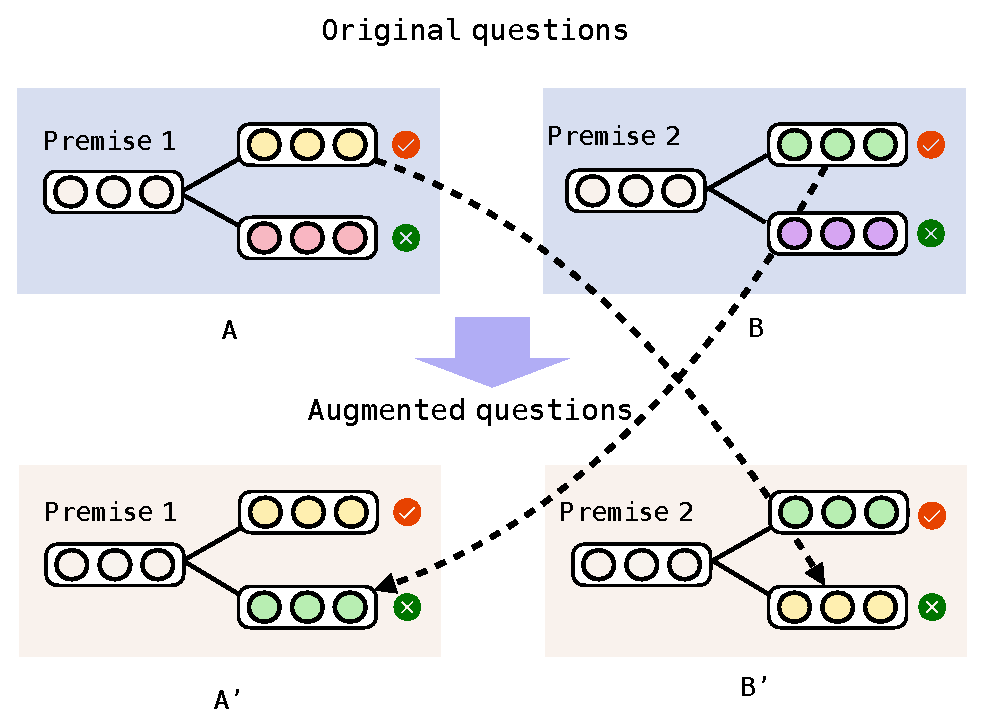
\includegraphics[width=\columnwidth]{figure/cross.eps}
\caption{The Crossover Operation: the true choice of both questions
are used to replace the false choices of these questions to create
two new proxy questions.}
\label{fig:cross}
\end{figure}

Compared to all other operations in classes 1 and 2, the crossover provides a proxy question that is most different from the original one but easier from a human perspective. This is because the two choices may be quite unrelated. If the model does not handle it correctly, it may be more indicative of a short circuit. As a result, the crossover is potentially a better short circuit test than others.

Another advantage of the crossover operation is that we can generate multiple false choices for an original question at a low cost, allowing us to test each original question more thoroughly. In contrast, most other operations cannot produce an adequate number of different variants of the original choice.

In summary, the proposed black-box choice operator provides a more generalizable and model-independent method for detecting short circuits in MCQ models. By applying various operations to create proxy questions, we can assess the model's performance and robustness more accurately, contributing to the development of better and more reliable models in the future.

\subsection{Improving Model Robustness by Data Augmentation}

If a model is shown to short-circuit by the proxy tests, its performance may decline, especially when applied to out-of-domain test data. To make models more robust, one natural thought is to generate more data to encourage models to focus on the relation between the premise and choices. While the operations used to generate proxy tests can also be utilized for data augmentation, not all of them are scalable or able to generate enough data for training.

The two operations that can generate a substantial amount of data are crossover and mutation. These operations can be applied to the training data to enhance the model's robustness.

\subsubsection*{Crossover for Data Augmentation}

Crossover is a good option for data augmentation because the two choices were originally true answers in their respective questions and presumably carry spurious features if the model was short-circuiting. By incorporating crossover into the training data, the model is forced to consider the premise in order to determine which choice is better.

\subsubsection*{Mutation for Data Augmentation}

Mutation has two flavors: (1) swap the words only in the true choice; (2) swap the words both in the true and the false choice. Compared to crossover, mutation has the potential to be more effective at improving model robustness. It not only forces the model to look into the premise due to its two very similar choices (same set of tokens), but also makes the model more sensitive to fine differences in word orders and enhances the model's prior grammatical knowledge.

\subsubsection*{Differentiating between Proxy Test and Data Augmentation}

It is essential to differentiate between the use of crossover and mutation operations in proxy tests and data augmentation. In proxy tests, these operations are used to modify the test data to assess the model's short-circuiting behavior. In contrast, when applied for data augmentation, the same operations work on the training data to enhance the model's robustness and generalization capabilities.

In conclusion, data augmentation through crossover and mutation operations can contribute to improving model robustness by encouraging models to focus on the relationship between the premise and choices. By incorporating these operations into the training data, models are forced to consider the premise and become more sensitive to the fine differences in word orders, leading to better performance and reliability in real-world applications.

\section{Implementation}
\label{sec:implement}

In this section we first attempt to experimentally 
determine the value for three key 
paramaters in our framework and then describe a baseline system for comparison
with our framework.
\cut{We also discuss the possibility to incorporate other data sources in building the co-occurrence matrix.}
%\subsection{Matrix Storage}
%As discussed in \secref{sec:enrich}, the co-occurrence matrix is very sparse
%because many pairs of Wikipedia concepts will not appear together in
%the Wikipedia corpus. Therefore instead of using a two-dimension array, we
%use a hash table to store the co-occurrence information. For each pair, we
%combine the IDs of the two Wikipedia concepts to form a key,
%and use the co-occurrence frequency as the value.

\subsection{Parameter Settings}
\label{sec:config}
The key parameters in our framework include $\tau$ which determines whether
to disambiguate a given term in our matrix enrichment process,
$W_c$, the co-occurrence window size in the iterations, and $W_s$, 
the sliding window size for wikifying new documents. 
%This subsection describes how these parameters
%are experimentally determined.

For threshold $\tau$, we randomly pick 100 paragraphs from Wikipedia corpus. We use function \emph{UpdateArticles} in
Algorithm \ref{enrich} to add links to these paragraphs using the matrixes
generated by the enrichment process on different thresholds.
We also manually add links to these 100 paragraphs, as ground truth labels.
We compare the different linking results with the ground truth then calculate the
precision and recall, which is shown in Table \ref{tab:theshold}.

\begin{table}[th]
\centering
\begin{tabular}{|c|c|c||c|c|c|}
\hline
$\tau$ & Precision & Recall & $\tau$ & Precision & Recall \\
\hline \hline
0.1 & 87.50\% & 40.94\% & \bf{0.5} & \bf{90.16\%} & 64.50\% \\
0.2 & 90.04\% & 63.66\% & 0.75 & 89.62\% & 66.01\% \\
0.25 & 89.29\% & 63.74\% & 0.875 & 88.89\% & 68.57\% \\
\hline
\end{tabular}
\caption{Result on Different Thresholds (with co-occurrence window $W_c$ = 15)}
\label{tab:theshold}
\end{table}
\cut{
\begin{table}[th]
\centering
\begin{tabular}{*{3}{|c}|}
\hline
Threshold & Precision & Recall \\
\hline \hline
0.1 & 87.50\% & 40.94\% \\
0.2 & 90.04\% & 63.66\% \\
0.25 & 89.29\% & 63.74\% \\
\bf{0.5} & \bf{90.16\%} & 64.50\% \\
0.75 & 89.62\% & 66.01\% \\
0.875 & 88.89\% & 68.57\% \\
\hline
\end{tabular}
\caption{Result on Different Thresholds (with co-occurrence window $W_c$ = 15)}
\label{tab:theshold}
\end{table}
}
We can see that threshold 0.5 achieves the best precision and also
reasonable recall. Since our matrix enrichment process is an
iterative process, precision in each iteration is more important, we
therefore choose 0.5 as threshold $\tau$.
%\KZ{Notice that $\tau$ is a
%parameter that affects the number of iterations at runtime.}

For $W_c$, we follow the same experiment described above,
since these two parameters are both used in the matrix generation part.
Instead of using different thresholds, we change the window size this
time. Table \ref{tab:window} shows the linking precision and recall 
using different $W_c$. 5 and 15 both achieve precision
higher than 90\%. To optimize the recall, we set $W_c = 15$.

\begin{table}[th]
\centering
\begin{tabular}{|c|c|c||c|c|c|}
\hline
$W_c$ & Precision & Recall & $W_s$ & Precision & Recall \\
\hline \hline
5 & 91.67\% & 45.20\% & 2 &84.59\%&	52.74\% \\
10 & 89.63\% & 60.84\% & 3 &84.95\%& 83.47\% \\
15 & 90.16\% & 64.50\% & 4 &85.52\%& 88.68\% \\
20 & 88.30\% & 67.05\% & 5 &85.55\%& 89.60\% \\
\hline
\end{tabular}
\caption{Result on Different $W_c$ and $W_s$ (with threshold $\tau$ = 0.5)}
\label{tab:window}
\end{table}

For $W_s$, we build another test data with 100 randomly picked paragraphs
from web and wikify them using the sliding window algorithm. The matrix used in
this experiment is generated by enriching 10,000 sample Wikipedia articles, 
with parameters $\tau= 0.5$ and $W_c=15$. Table \ref{tab:window} compares 
the results on different $W_s$ with the manually created ground truth.
Both precision and recall increase with growing $W_s$. 
When $W_s$ is larger than 5, the whole process takes too much time and 
is thus not practical. Consequently we set $W_s = 5$.

%\begin{table}[th]
%\centering
%\begin{tabular}{*{3}{|c}|}
%\hline
%$W_s$ & Precision & Recall \\
%\hline \hline
%2 &84.59\%&	48.12\% \\
%3 &84.95\%&	72.72\% \\
%4 &85.52\%&	77.10\% \\
%5 &85.55\%&	77.82\% \\
%\hline
%\end{tabular}
%\caption{Result on Different $W_s$}
%\label{tab:windows}
%\end{table}
\cut{
\subsection{Boosting of Common Terms}
One challenge we discuss in \secref{intro} is that some common and
``easier'' terms are usually less linked than popular and
``difficult'' terms.
%This biased distribution of links affects our overall iteration results.
%When these terms appear in an article, it is more likely it bears
%the most general sense.
For example, when ``Country'' appears in an article,
its sense is usually the general one, which means a region legally
identified as a distinct entity in political geography.
Less often does it mean ``Country music''.
However, in the Wikipedia corpus, the term ``Country'' is rarely linked to
its general sense because it's not ``link-worthy''.
Consequently, our iteration process is not likely to link such common terms
to their general senses, either.
Instead, common terms can be mis-linked to their special senses.

To avoid this problem, we apply the following approach to ``boost'' the most
general sense of common terms.
For each term in the original corpus, we count the number of times
it is unlinked vs. linked. We compute a ratio
\[r = \frac{f(unlinked)}{f(linked)+f(unlinkded)}
\]
between the unlinked frequency and the sum of unlinked frequency and linked frequency.
Our assumption is that, the higher this ratio is, the more
likely this term is using its general sense.
Subsequently we adapt $S_{CC}$ in
\secref{sec:enrich} to:
\[ {S_{CC}}^\prime\left(c\right)=\left\{
\begin{array}{r@{\;\;}l}
g\left(r\right)\cdot S_{CC}\left(c\right) & \mbox{if c is a general sense}\\
g\left(1-r\right)\cdot S_{CC}\left(c\right) & \mbox{if c is not a general sense}
\end{array} \right.
\]
where $r$ act as a boost factor for the general sense
when the term is a common one, $g$ is a monotonically increasing
function of $r$ that adjusts the impact of boosting.

To discover function $g$, we sample 10,000 articles from Wikipedia corpus then count the
linked frequency and unlinked frequency of each terms. We sort all the terms based
on $r$. According to our observation, only terms with extremely high $r$ are likely
to be ``easier'' terms. For example, ``year'', with $r$ equals to 0.999, is
usually used as a time unit, which is its common sense. However, ``apple'',
with $r$ equals to 0.863, is usually used in the senses of a kind of fruit
and a technology company. Thus, we fit function
$g$ shown in \figref{fig:gfun}. The intuition is to give those terms with very
high $r$ (nearly 1) a boost.

\begin{figure}[th]
\centering
\epsfig{file=figure/gfunction.eps,width=0.6\columnwidth}
\caption{Function $g$}
\label{fig:gfun}
\end{figure}
}
\subsection{Baseline System}
Besides the algorithm introduced in \secref{sec:framework},
for comparison purpose,
we also implemented a baseline system which wikifies a document by the
co-occurrence between Wikipedia concepts and plain words.
This system can be thought of as a direct port of WSD from using WordNet to
using Wikipedia, and it also uses a common bag-of-words approach.
In this baseline system, the co-occurrence vector of
each Wikipedia concept is constructed
from words and frequencies in the article of this concept itself.
With the vectors of all Wikipedia concepts,
we can wikify a document by comparing the co-occurrence vectors with
the context of each term in the document. Given a document, we parse it
into terms in the same way as our wikification framework.
Each term has a list of candidate Wikipedia concepts.
We compute the cosine similarity
between the vector of each candidate concept and the vector built from
the input document. The concept whose vector has the best similarity with
the document vector is chosen to disambiguate that
term. We compare the result of this baseline system with
our wikification framework in \secref{sec:eval}.

%\subsection{Beyond the Wikipedia Corpus}
In this paper, Wikipedia acts as a lexicon which provides all the
surface terms as well as concepts to link to for wikification.
However, even though the Wikipedia text
corpus itself is very large, it is unlikely to contain all the co-occurrence
information there is between any two concepts. Additional data sources maybe
used to provide co-occurrence evidences not seen in Wikipedia itself.
For example, suppose in the Wikipedia corpus, concepts $a$ and $b$ co-occur,
concepts $a$ and $c$ also co-occur, but there's no evidence which supports
the co-occurrence of $b$ and $c$. Now, given a new plain text document, because of the co-occurrence between $a$ and $b$ and the co-occurrence between $a$ and $c$,
we may be able to disambiguate three terms $t_a$, $t_b$ and $t_c$ to $a$, $b$,
and $c$, respectively in the document. Consequently, a new occurrence ($b$, $c$)
which was never seen in Wikipedia itself, can be discovered and added to our
co-occurrence knowledge.
%Not only Wikipedia corpus, we also consider the possibility to bring in
%other source to help us collect more co-occurrence information. Plain
%text on web is a candidate. We are interested in the word and phrase
%distribution on both Wikipedia article and plain text.

We conduct the following experiment to verify our hypothesis.
We randomly sample 10,000 web pages from a Bing snapshot and
extract plain text from them.
Then we randomly pick two groups of 10, 000 Wikipedia articles, called
Wiki-1 and Wiki-2. We compute the word distribution and the Wikipedia terms
(phrase) distributions from these three groups of text and measure the
the cosine similarity between word distributions and between
phrase distributions in Table \ref{tab:vector}.

\begin{table}[th]
\centering
\begin{tabular}{|c|c|c|}
\hline
Data Sources           &  Word Similarity &  Phrase Similarity \\
\hline \hline
Wiki-1 vs. Wiki-2 &      0.992 &       0.990 \\
Plain text vs. Wiki-1 &      0.633 &      0.765 \\
Plain text vs. Wiki-2 &      0.629 &      0.764 \\
\hline
\end{tabular}
\caption{Word and Phrase Distribution Similarity}
\label{tab:vector}
\end{table}

Table \ref{tab:vector} shows that the word and phrase distribution
between two Wikipedia sets are very similar.
Whereas both word and phrase distribution of plain text share lower
similarity with those of the two Wikipedia sets. This indicates that
data sources outside of Wikipedia do have significant differences and hence
have the potential of introducing fresh co-occurrence information into
the Wikipedia corpus.

One straightforward way of incorporating the co-occurrence data from other sources
into Wikipedia is to wikify the plain text,
calculate co-occurrence frequency between the concepts inside a window, and then
update that information into the co-occurrence matrix we obtained from
Wikipedia itself.
We use the matrix generated from 10,000 sample Wikipedia articles to wikify
10,000 other web pages. Results show that this process introduces 2,802,392
fresh pairs, which is 10.47\% of the original matrix size.

%Our iterative algorithm that enrich the co-occurrence matrix can not only
%be applied on Wikipedia articles, but also plain text, which can bring us
%more knowledge. The process is similar to what we use to wikify plain text
%document. We set a sliding window and calculate the ($S_{SW}$)s. But instead
%of finding the best sense for each term, we delete the worst sense in each
%iteration with the lowest sum of ($S_{SW}$)s.
%
%The whole process on plain text starts with an initial co-occurrence matrix,
%which can be generated by the process on Wikipedia articles. In each iteration,
%each existing sense of a term is assigned a value which is the sum of all the
%($S_{SW}$)s this sense contributes to. The sense with the lowest value is deleted.
%Once there is only one sense left for a term, or to say the sense of that term
%is fixed, we add a link to the corresponding document and update the co-occurrence
%matrix. The iterations continue until no link can be added.



\section{Evaluation}
\label{sec:evaluation}
Through the above approach, we translate two popular English knowledge graphs: \con and \pro into \zhcon and \zhpro, respectively. In terms of the word embedding, we use the Chinese Wikipedia dump on Aug 1, 2018,  to train word embedding with Word2Vec, where the vocabulary size is 110,978 and the embedding dimension is 300.\footnote{\url{https://code.google.com/archive/p/word2vec/}}
In this section, we evaluate the coverage and accuracy of \zhcon and \zhpro, respectively. The baseline experiment we choose is the direct translation using the translator, and we will denote it as \textbf{DT} later. For example, in the baseline, we translate triple (``ball'', AtLocation, ``ballroom'') by feeding ``ball, ballroom'' into translator, and split the translation result ``球, 舞厅'' into (``球'', AtLocation, ``舞厅'') as the final translation result. Here, we do not provide the translator with the contextualized sentence such as ``the ball is at the ballroom.'', since there are no fixed patterns in the translated sentence, which makes it hard to extract the corresponding part, even for the translated results of one particular relation.\footnote{For example, although ``french chefs are capable of preparing food.'' and ``spider web is capable of catching morning dew.'' share the same structure in English, they will be translated into ``法国厨师有能力准备食物。'' and ``蜘蛛网能够吸引晨露。'' respectively, which requires more than one pattern to split the translation result.}

%\KZ{In addition to the end-to-end eval on the two translated KBs, you also
%need to do some ablation tests. For example, what if you don't do the revision?
%Is there any alternative ways to do revision? You need to show that your way of
%revision is better than straightforward methods.}

\subsection{\zhcon}
\zhcon is a mixed Chinese common sense knowledge graph, which comes from two sources, 
the original Chinese part of \con and the translation result of the English part of \con.

\textbf{Coverage.}
As shown in Table \ref{tab:zh_conceptnet_coverage}, the size of \zhcon is \textbf{4.76} times as large as the original Chinese part of \con, 
which is a substantial increase in quantity. The size of \zhpro is not as 4.91 times as we expected, since there exists overlap in the process of merging.
To our best knowledge, there are no other Chinese knowledge graphs dedicated to common sense, and \zhcon will be the first large one with about 2 million edges, which, we hope, could be a valuable asset for Chinese common sense research.
\begin{table}[ht]
\caption{Size of \zhcon.}
\label{tab:zh_conceptnet_coverage}
\centering
\begin{tabular}{ll}\hline 
\textbf{Dataset}&\textbf{Size}\\\hline
1. Original Chinese Part in \con &438,307(x1.00)\\  
2. Translated English part in \con &1,716,327(x3.91)\\
\zhcon (Merge 1 and 2)&\textbf{2,085,681(x4.76}) \\\hline
\end{tabular}
\end{table}

\textbf{Accuracy.}
To evaluate the quality of \zhcon, 
we randomly sample 500 samples from original Chinese part in \con, 
\text{DT} result of English part in \con, translation result of English part in \con based on our two-steps approach (we denote it as \textbf{OURS} later), and \zhcon (which merges the Chinese part in \con and translated English part in \con of \textbf{OURS}), respectively. 
We ask two annotators to evaluate these samples. 
As Table \ref{tab:conceptnet_accuracy} shows, there exists 1\% error in the original Chinese part of \con, which comes from crowdsourcing errors.
%Since approximately 86\% of the data in \con comes from collaborative datasets, such as Wiktionary, DBpedia, etc 
Compared with the direct translation (\text{DT}), the accuracy of the translation result based on \textbf{OURS} has a relative gain of \textbf{2.8\%}.
The accuracy of \zhcon has also been improved to \textbf{89.6\%} due to the high quality of the merged original Chinese part from \con.

\begin{table}[ht]
\caption{Accuracy of different approaches. The Kappa coefficients \cite{landis1977measurement} of two annotators suggest a substantial agreement.}
\label{tab:conceptnet_accuracy}
\centering
\begin{tabular}{ll}\hline
	Approach & Accuracy (Kappa) \\ \hline
	1. Original Chinese part in Conceptnet& 98.3\%(0.58) \\
	2. \textbf{DT} of English part                 & 84.5\%(0.85) \\
	3. \textbf{OURS} & 87.3\%(0.85) \\
	Zh-Conceptnet (Merge 1 and 3) & \textbf{89.6\%(0.79)} \\\hline
\end{tabular}
\end{table}

\textbf{Qualitative Results.}
Our approach can handle some intractable word sense disambiguations, such as ``date'', ``ball'', ``court'', ``capital'', ``fan'', etc, as shown in the blue part in Table \ref{tab:zh_conceptnet_case}.
Besides, our method can translate (``fan'', RelatedTo, ``sector'') into (``扇'', RelatedTo, ``扇形''), while the result of \textbf{DT} is (``粉丝'', RelatedTo, ``部门''). This shows that our approach can disambiguate ``fan''  and ``sector'' at the same time. As for the errors in \zhcon, according to our observations, most errors in \zhcon come from the triples with the relation of ``RelatedTo''. Since the relation of ``RelatedTo'' is relatively weak in English such as (``blunt'', RelatedTo, ``money''), it becomes even weaker after translation, and the triples with the relation of ``RelatedTo'' account for 48.16\% of all the triples in \con. The red part in Table \ref{tab:zh_conceptnet_case} shows more error cases. 


\begin{table}[!htbp]
\caption{Some examples triples in \zhcon. Correct translations are in {\color{blue} blue}, and incorrect ones are in {\color{red}red}.}
\label{tab:zh_conceptnet_case}
\resizebox{\linewidth}{!}{%
\begin{tabular}{lll}\hline
	\textbf{English}                 & \textbf{OURS}     & \textbf{DT}  \\\hline
	{\color{blue}(date, fruit)/IsA}                  & {\color{blue}枣, 水果}     & {\color{blue}时间, 水果}    \\ 
	{\color{blue}(ball, ballroom)/AtLocation}        & {\color{blue}舞会, 舞厅}    & {\color{blue}球, 舞厅}     \\ 
	{\color{blue}(can, shelf)/AtLocation}            & {\color{blue}罐头, 货架}    & {\color{blue}可以, 货架}    \\ 
	{\color{blue}(court, gymnasium)/AtLocation}       & {\color{blue}球场, 体育馆}   & {\color{blue}法院, 体育馆}   \\ 
	{\color{blue}(munition, arm)/MannerOf}            & {\color{blue}军火, 武装}    & {\color{blue}军火, 手臂}    \\ 
	{\color{blue}(capital, proper noun)/AtLocation} & {\color{blue}大写, 专有名词}  & {\color{blue}资本, 专有名词}  \\ 
	{\color{blue}(spinach, can)/RelatedTo}             & {\color{blue}菠菜, 罐头}    & {\color{blue}菠菜, 可以}    \\ 
	{\color{blue}(fan, blow)/RelatedTo}             & {\color{blue}扇子, 吹}    & {\color{blue}粉丝, 吹}    \\ 
	{\color{blue}(fan, peacock)/RelatedTo}             & {\color{blue}扇子, 孔雀}    & {\color{blue}粉丝, 孔雀}    \\ 
	{\color{blue}(fan, sector)/RelatedTo}             & {\color{blue}扇, 扇形}    & {\color{blue}粉丝, 部门}    \\ 
	{\color{blue}(collection, garage)/AtLocation}             & {\color{blue}珍藏, 车库}    & {\color{blue}集合, 车库}    \\ 
	{\color{blue}(brook, tolerate)/RelatedTo}             & {\color{blue}容忍, 姑息}    & {\color{blue}小溪, 容忍}    \\ 
	{\color{red} (blunt, money)/RelatedTo}             & {\color{red} 生硬, 钱}    & {\color{red} 生硬, 钱}    \\ 
	{\color{red} (fouta, thin)/RelatedTo}             & {\color{red}伏塔加, 瘦}    & {\color{red}富塔, 瘦}    \\ 
	{\color{red}(major ninth, interval)/RelatedTo}             & {\color{red}主要的第九, 间隙}    & {\color{red}主要的第九, 间隔}    \\ 
	{\color{red}(melo, music)/RelatedTo}             & {\color{red}甜瓜, 音乐}    & {\color{red}melo, 音乐}    \\ \hline
\end{tabular}}
\end{table}

%粉丝    /r/RelatedTo    打击
%fan     ['球迷', '迷', '风扇', '扇子', '扇', '粉丝']
%blow    ['打击', '吹', '刮']
%扇子    吹      0.29190982571468305
%(fan, blow)/RelatedTo             & 扇子, 吹    & 粉丝, 吹    \\ \hline
%
%粉丝    /r/RelatedTo    孔雀
%fan     ['球迷', '迷', '风扇', '扇子', '扇', '粉丝']
%peacock ['孔雀']
%扇子    孔雀    0.2387474142191117
%(fan, peacock)/RelatedTo             & 扇子, 孔雀    & 粉丝, 孔雀    \\ \hline
%
%粉丝    /r/RelatedTo    部门
%fan     ['球迷', '迷', '风扇', '扇子', '扇', '粉丝']
%sector  ['扇形', '部门']
%扇      扇形    0.2658884528019793
%(fan,sector)/RelatedTo             & 扇, 扇形    & 粉丝, 部门    \\ \hline
% 
%\begin{table}[th]
%\caption{Some examples triples in \zhcon}
%\label{tab:conceptnet_case}
%\center
%\begin{tabular}{|l|l|l|}\hline
%\textbf{Node1(Subject)} & \textbf{Relation} & \textbf{Node2(Object)} \\ \hline\hline
%	\begin{tabular}[c]{@{}l@{}}植物/plant\end{tabular} & /r/Desires & 水和太阳/water\_and\_sun \\ \hline
%	\begin{tabular}[c]{@{}l@{}}植物/plant\end{tabular} & /r/AtLocation & \begin{tabular}[c]{@{}l@{}}污垢/dirt,\\花盆/flower\_pot,\\花园/garden\end{tabular} \\ \hline
%	
%	\begin{tabular}[c]{@{}l@{}}植物/plant\end{tabular} & /r/Antonym & \begin{tabular}[c]{@{}l@{}}矿物/mineral,\\动物/animal\end{tabular}\\ \hline
%	
%	\begin{tabular}[c]{@{}l@{}}植物/plant\end{tabular} & /r/NotCapableOf & \begin{tabular}[c]{@{}l@{}}移动/move,\\跑/run,\\想想/think,\\走路/walk\end{tabular} \\ \hline
%	
%	\begin{tabular}[c]{@{}l@{}}工厂/plant\end{tabular} & /r/RelatedTo & \begin{tabular}[c]{@{}l@{}}设施/facility,\\制造业/manufacturing,\\起动器/starter\\机械/machinery\end{tabular} \\ \hline
%	%					工厂(factory)\\/plant & /r/IsA & \begin{tabular}[c]{@{}l@{}}包装厂/packinghouse,回收厂/recycling\_plant,\\ 炼油厂/refinery\end{tabular} \\ \hline
%	\begin{tabular}[c]{@{}l@{}}植物/plant\end{tabular} & /r/CapableOf & \begin{tabular}[c]{@{}l@{}}绽放/bloom,\\成长/grow,\\光合作用/photosynthesis\end{tabular}  \\\hline
%\end{tabular}
%\end{table}

\subsection{\zhpro}
We translate \pro into \zhpro based on our proposed approach. In this section, we compare \zhpro with two well-known Chinese taxonomic knowledge graphs CN-Probase \cite{Xu2017} and zhishi.me \cite{Niu2011} in terms of coverage and accuracy.

\textbf{Coverage.}
As shown in Table \ref{tab:zh_probase_coverage}, \zhpro has the same order of magnitude as CN-Probase and is \textbf{11.74} times larger than zhishi.me. 
We further evaluate the overlap between \zhpro and existing Chinese taxonomic knowledge graphs.
Since CN-Probase is not open-source, to calculate the ratio of overlap, we apply the method of sampling. First, we sample 500 ``IsA'' pairs from CN-Probase via the public API of CN-Probase and count the ratio of overlap with \zhpro, which is only \textbf{1\%}. Then, we sample 500 ``IsA'' pairs from \zhpro, and get the ratio of \textbf{6\%}. The intersection of \zhpro and zhishi.me is only \textbf{5,243} pairs.
The reasons why the overlap ratio between \zhpro and CN-Probase is small are as follows: First, as shown in Table \ref{tab:zh_probase_coverage}, CN-Probase has more instances and fewer concepts, like the shape of the Pyramid, while \zhpro has more concepts and fewer instances, like the shape of the inverted Pyramid. 
Second, most entities in \zhpro are translated from English, which only exist in English context, while entities in CN-Probase are extracted from the high-quality Chinese encyclopedia. The third reason is that many latest entities are collected in CN-Probase, while not in \zhpro, since the publish time of CN-Probase is later.
Due to the small overlap between \zhpro and existing Chinese taxonomic knowledge graphs, \zhpro can substantially enrich them. Also, due to the large concept space and broader topics, it will exhibit a stronger ability in capturing the implied semantics, as demonstrated in \cite{wang2010toward}.
Therefore, we can conclude that although the number of ``IsA" pairs in CN-Probase is 3 times larger than that in \zhpro, \zhpro can still greatly enrich existing Chinese taxonomic knowledge graphs.

%The ratio of pairs in CN-Probase, which are also in \zhpro, is \textbf{6\%}, while the ratio of ``IsA'' pairs in \zhpro, which are also in CN-Probase, is less than \textbf{1\%}. This is the sampling estimate via the public API interface of CN-Probase, since it is not open-source.
%The size of the concepts in \zhpro (2,094,825) is \textbf{8} times larger than that in CN-Probase (270,000) while the number of the instances of \zhpro (4,532,110) is much less than CN-Probase (17,000,000). The reason may be that the data sources of both CN-Probase and zhishi.me come from Baidu Baike, Hudong Baike and Chinese Wikipedia (three largest Chinese encyclopedia websites), which, more specifically, come from the well-formed information, such as abstract, infobox, category information, therefore, the instance space of these two knowledge graphs is extremely large while the concept space is relatively small. 
%For example, in CN-Probase, the top instances of concept ``人/person'' are always specific person names, such as ``曹操'', ``崔健'', ``李清云'', etc.
%In contrast, the data source of \pro is massive text corpora in online webpages, which is freer than the data source of CN-Probase, thus, its concept space is large.
%For example, the top instances of concept ``人/person'' in \zhpro are all sub-concepts, such as ``老人/old people'', ``朋友/friend'', ``医生/doctor'', etc.


%\KZ{The style and font size of all tables must be consistent. You can't use 
%resizebox to scale everything into one column so that the fontsizes are
%different.}
\begin{table}[ht]
\caption{Size of existing taxonomic knowledge graphs. (`-' means we cannot get it. ``con-ins'' means ``concept-instance''. ``con-subc'' means ``concept-subconcept''.)}
\label{tab:zh_probase_coverage}
\centering
\begin{tabular}{cccc}\hline
	\textbf{}&\textbf{\zhpro}&\textbf{CN-Probase}&\textbf{zhishi.me}\\ \hline
	concepts  &\textbf{2,094,825}&270,000&17,936\\
	instances  &4,532,110&17,000,000&511,667\\
	con-ins pairs &\textbf{7,054,382}&-&959,581\\
	con-subc pairs&\textbf{4,238,111}&-&2,003\\
	IsA pairs&11,292,493&33,000,000&961,587 \\ \hline
	\end{tabular}
\end{table}

\textbf{Accuracy.}	
To evaluate the quality of \zhpro, 
we randomly sample 500 samples from \pro, \textbf{DT} result of \pro, translation result based on \textbf{OURS}, respectively.
We ask two annotators to evaluate these samples. 
The results are shown in Table \ref{tab:probase_accuracy}. 
Compared with \textbf{DT}, the accuracy based on \textbf{OURS} has increased by \textbf{1.4\%} (from 85.2\% to 86.6\%).
It is less than the improvement (2.8\%) of translation result based on \textbf{OURS} in
\zhcon, because most nodes in \pro are less ambiguous multi-words.
In addition to the inherent error around 7\% (accuracy 93.0\%) in \pro, our translation approach only introduces an additional error of 6.4\% (accuracy 86.6\%), which will be analyzed in the next section. 
\begin{table}[ht]
\caption{The accuracy of existing Chinese taxonomic graphs. The Kappa coefficients of two annotators suggest the substantial agreement.  }
\label{tab:probase_accuracy}
\centering
\begin{tabular}{ll}\hline
	\textbf{Knowledge Graph} & \textbf{Accuracy(Kappa)} \\ \hline 
	\pro    & 93.0\%(0.75) \\ 
	\textbf{DT} of \pro    & 85.2\%(0.84) \\ 
	Zh-Probase & 86.6\%(0.88) \\ 
	CN-Probase     & 95.0\% \\ 
	zhishi.me     & 100\% \\ \hline
\end{tabular}
\end{table}

\textbf{Qualitative Results.}
Our approach can handle some intractable word sense disambiguations, such as ``bank'', ``bark'', ``scale'' etc, as shown in the blue part in Table \ref{tab:probase_case}. On the other hand, there also exist some errors introduced by our method. 
Typical error cases are shown in the red part in Table \ref{tab:probase_case}. According to our observation, most of the errors come from two sources. 
First, translating the entities directly leads to ambiguous Chinese results.
For example, (``go move shift'', IsA, ``song'') will be translated into (``去转移'', IsA, ``歌曲''), which is hard to understand in Chinese. However, translation of named entities is hard to be avoided because not all the first letter of named entities will be capitalized.
Second, the machine translator sometimes cannot return all the Chinese word senses of the word. For example, (``florist'', isA, ``outlet'') will be incorrectly translated into (``花商'', isA, ``出口'') because the translator does not return the Chinese word sense ``批发商店'', which is the correct Chinese word sense of ``outlet'' here.

\begin{table}[!htbp]
	\caption{Some ``IsA'' samples in \zhpro. Correct translations are in {\color{blue} blue}, and incorrect ones are in {\color{red}red}.}
	\label{tab:probase_case}
	\resizebox{\linewidth}{!}{%
		\begin{tabular}{lll}\hline
			\textbf{English}                            & \textbf{OURS}     & \textbf{DT} \\\hline
			{\color{blue} (bank, natural feature)}          & {\color{blue}岸边, 自然特征} & {\color{blue}银行, 自然特征} \\
			{\color{blue}(bank, man-made boundary)}        &  {\color{blue}岸边, 人造边界}  & {\color{blue}银行, 人造边界}  \\
			{\color{blue}(grand Arab capital, capital)}    & {\color{blue}阿拉伯首都, 首都} & {\color{blue}阿拉伯首都, 资本} \\
			{\color{blue}(spring, natural water)}          & {\color{blue}泉水, 天然水}   &  {\color{blue}春天, 天然水}   \\
			{\color{blue}(spring, surface water)}          & {\color{blue}泉水, 地表水}   &  {\color{blue}春天, 地表水}   \\
			{\color{blue}(bark, close range vocalization)}&{\color{blue}吠,近距离发声}&{\color{blue}树皮,近距离发声}\\
			{\color{blue}(bark, vocalization)}&{\color{blue}吠,发声}&{\color{blue}树皮,发声}\\
			{\color{blue}(scale, graphic learning material)}&{\color{blue}比例尺, 图形学习材料}&{\color{blue}规模, 图形学习材料}\\
			{\color{blue}(scale, voice exercise)}&{\color{blue}音阶, 语音练习}&{\color{blue}规模, 语音练习}\\
			{\color{blue}(scale, animal covering)}&{\color{blue}鳞, 动物覆盖}&{\color{blue}规模, 动物覆盖}\\
			{\color{blue}(scale, musicianship skill)}&{\color{blue}音阶, 音乐技巧}&{\color{blue}规模, 音乐技巧}\\
			{\color{blue}(ball, social event)}&{\color{blue}舞会, 社交活动}&{\color{blue}球, 社交活动}\\
			{\color{blue}(ball, physical activity)}&{\color{blue}舞会, 体力活动}&{\color{blue}球, 身体活动}\\
			{\color{blue}(ball, celebration)}&{\color{blue}舞会, 庆祝}&{\color{blue}球, 庆祝}\\
			{\color{blue}(fan, artifact)}&{\color{blue}扇子, 人工制品}&{\color{blue}粉丝, 人工制品}\\
			{\color{red}(florist, outlet)}&{\color{red}花商, 出口}&{\color{red}花店, 出口}\\
			{\color{red}(go move shift, song)}&{\color{red}去移动, 鸣声}&{\color{red}转移, 歌曲}\\
			{\color{red}(Banks of the Ohio, song)}&{\color{red}俄亥俄州的银行, 曲子}&{\color{red}俄亥俄州的银行, 歌}\\
			{\color{red}(chin check, song)}&{\color{red}下巴检查, 鸣声}&{\color{red}下巴检查, 歌}\\\hline
		\end{tabular}
	}
\end{table}

%\subsection{Discussion of First step of \textbf{OURS}}
%%probase 22 16
%%probase 26 12  4770716/11292493=0.422
%total error:
%probase 11\%,13\%    ave:12\%
%
%-inner error
%probase 3\%, 7\%    ave:5\%
%
%%%%%%%%conceptnet 200 43 11  241962/2085681=0.116
%
%%conceptnet 200 15  3
%%conceptnet 200 28 9  241962/2085681=0.116
%total error:
%conceptnet 7.5\%,14\%  ave:10.75\%
%-inner error
%conceptnet 6\%, 9.5\%  ave:7.75\%
%
%hj:
%conceptnet 2,3,4:19,3,8
%probase 2,3,4: 22,16,7
%xr:
%conceptnet 2,3,4:27,9,12
%probase 2,3,4: 22,8,9
%
%
%wsd:
%conceptnet  5.5\%,7.5\% ave: 6.5\%
%probase: 7.5\%,6.5\% ave:7\%


%\begin{table}[H]
%\caption{Some ``IsA'' samples in \zhpro}
%\label{tab:probase_case}
%\begin{tabular}{|l|l|l|}
%	\hline
%	\textbf{Instance} & \textbf{Subconcept} & \textbf{Concept} \\ \hline\hline
%	\begin{tabular}[c]{@{}l@{}}番茄(tomato)\\玉米(maize, corn)\\大豆(soy, soybean)\end{tabular} & 
%	\begin{tabular}[c]{@{}l@{}}植物\\(plant, flora)\end{tabular} &
%	\begin{tabular}[c]{@{}l@{}}有机体(organism)\\ 生产者(producer)\end{tabular} \\ \hline
%	
%	%		\begin{tabular}[c]{@{}l@{}}无水乙醇/(anhydrous ethyl alcohol)\\ 合成乙醇/(synthetic ethyl alcohol)\end{tabular} & 
%	%		\begin{tabular}[c]{@{}l@{}}乙醇\\(alcohol,ethanol)\end{tabular}&
%	%	    \begin{tabular}[c]{@{}l@{}}生物燃料/(biological fuel)\\ 有机溶剂/(organic solvent)\\ 化合物/(compound)\end{tabular} \\ \hline
%	
%	\begin{tabular}[c]{@{}l@{}}橡胶厂(rubber plant)\\
%		炼油厂(oil refinery)\\ 电厂(power plant)\end{tabular} & \begin{tabular}[c]{@{}l@{}}工厂\\(factory, mill)\end{tabular} & \begin{tabular}[c]{@{}l@{}}资产(asset)\\地方(spot,place)\end{tabular} \\ \hline
%	
%	\begin{tabular}[c]{@{}l@{}}狗(dog),猫(cat,feline)\\ 牛(cattle,cow,ox)\end{tabular} &
%	\begin{tabular}[c]{@{}l@{}} 动物\\(animal)\end{tabular} & \begin{tabular}[c]{@{}l@{}}类别(category)\\
%		主题(theme)\\ 
%		生物(creature)\end{tabular}\\ \hline
%\end{tabular}
%\end{table}

%
%近距离发声      IsA     树皮
%close range vocalization        ['近距离发声']
%bark    ['吠', '树皮']
%近距离发声      吠      0.22152851973712392
%近距离发声      树皮    0.07381855955982522
%(bark, close range vocalization)&吠,近距离发声&树皮,近距离发声\\\hline
%
%发声    IsA     树皮
%vocalization    ['发声']
%bark    ['吠', '树皮']
%发声    吠      0.20266486701662512
%发声    树皮    0.02289122701292446
%(bark, vocalization)&吠,发声&树皮,发声\\\hline
%
%图形学习材料    IsA     规模
%graphic learning material       ['图形学习资料', '图形学习材料']
%scale   ['音阶', '规模', '级别', '尺度', '鳞', '比例', '比例尺']
%图形学习材料    比例尺  0.268557394974322
%图形学习材料    尺度    0.21657940353240107
%(scale, graphic learning material)&比例尺, 图形学习材料&规模, 图形学习材料\\\hline
%
%语音练习        IsA     规模
%voice exercise  ['配音练习', '语音练习']
%scale   ['音阶', '规模', '级别', '尺度', '鳞', '比例', '比例尺']
%语音练习        音阶    0.31595054519851007
%(scale, voice exercise)&音阶, 语音练习&规模, 语音练习\\\hline
%
%动物覆盖        IsA     规模
%animal covering ['动物覆盖物', '动物覆盖']
%scale   ['音阶', '规模', '级别', '尺度', '鳞', '比例', '比例尺']
%动物覆盖        鳞      0.2980978974505864
%动物覆盖        尺度    0.2653591599617439
%(scale, animal covering)&鳞, 动物覆盖&规模, 动物覆盖\\\hline
%
%音乐技巧        IsA     规模
%musicianship skill      ['音乐才能', '音乐技巧']
%scale   ['音阶', '规模', '级别', '尺度', '鳞', '比例', '比例尺']
%音乐技巧        音阶    0.3543777738132791
%(scale, musicianship skill)&音阶, 音乐技巧&规模, 音乐技巧\\\hline
%
%社交活动        IsA     球
%social event    ['社交活动']
%ball    ['球', '舞会', '丸子']
%社交活动        舞会    0.5062901630643256
%(ball, social event)&舞会, 社交活动&球, 社交活动\\\hline
%
%身体活动        IsA     球
%physical activity       ['体力活动', '身体活动']
%ball    ['球', '舞会', '丸子']
%身体活动        舞会    0.30998053650136403
%体力活动        舞会    0.2693407790252701
%(ball, physical activity)&舞会, 体力活动&球, 身体活动\\\hline
%
%庆祝    IsA     球
%celebration     ['庆典', '典礼', '庆祝']
%ball    ['球', '舞会', '丸子']
%庆典    舞会    0.5391221765807583
%(ball, celebration)&舞会, 庆祝&球, 庆祝\\\hline
%
%每日文章        IsA     粉丝
%everyday article        ['日常用品', '每日文章']
%fan     ['扇子', '爱好者', '球迷', '风扇', '迷', '粉丝']
%日常用品        扇子    0.24773631914892047
%每日文章        爱好者  0.19835457168625464
%(fan, everyday article)&扇子, 日常用品&粉丝, 每日文章\\\hline
%
%人工制品        IsA     粉丝
%artefact        ['假象', '人工制品']
%fan     ['扇子', '爱好者', '球迷', '风扇', '迷', '粉丝']
%人工制品        扇子    0.09307627931322751
%(fan, artefact)&扇子, 人工制品&粉丝, 人工制品\\\hline

\section{Related Work}
This section surveys previous works on question generation and tree encoding
respectively.

Text question generation has attracted the attention 
after the work of ~\citeauthor{du2017learning}~\shortcite{du2017learning}, who uses deep seq2seq model 
to generate questions from a raw text paragraph. 
Before that, text question generation relied heavily on hand-craft 
question patterns~\cite{HeilmanS10,LabutovBV15,MostowC09} which is time and 
labor consuming. 

However, this pure seq2seq model is not focused and 
has no control over part in the paragraph to generate question. 
~\citeauthor{zhou2017neural}~\shortcite{zhou2017neural} proposed to encode 
key phrase information using binary indicators to generate 
key-aware questions and they assumes the answer to be key phrase. 
Considering key phrase (answer) is unavailable in reality, 
~\citeauthor{SubramanianWYT17}~\shortcite{SubramanianWYT17} applied 
a two-stage approach. First, key phrases are extracted by 
pointer network~\cite{ptrnet}. Second, 
key phrases are encoded in the same way as 
Zhou et al. With the intuition that questions could be asked in many ways, 
~\citeauthor{Yao2018vae}~\shortcite{Yao2018vae} used conditional-VAE to 
increase the diversity of questions. More recently, models with 
auxiliary feature information~\cite{HarrisonW18} helped improve 
the question quality. Structure question generation aims at 
converting structured data such as triples in knowledge graph to questions. 
~\citeauthor{SerbanGGACCB16}~\shortcite{SerbanGGACCB16} proposed a model to generate factoid questions from knowledge base triples.  None of the above work
considered using parse tree structures to aid question generation process,
which is the focus of this paper.

Sequential RNN model takes sentence as a sequence of words, 
ignoring the syntactic information. In order to utilize
such syntactic information with sequential information, 
~\citeauthor{tai2015improved}~\shortcite{tai2015improved} proposed Tree-LSTM to 
encode the binary parse tree recursively in a bottom-up fashion to 
classify sentiment. In text generation task, 
\citeauthor{eriguchi2016tree}~\shortcite{eriguchi2016tree} 
proposed a tree-to-sequence model with attention mechanism to do 
machine translation and 
~\citeauthor{liang2018automatic}~\shortcite{liang2018automatic} proposed a 
tree-to-sequence model which could handle arbitrary trees, 
to do code comment generation. Our work is inspired by these previous
attempts and we are first to adapt structure encoded neural models to
textual question generations.
\section{Conclusion}
\label{sec:conclude}
In this work,
we propose a new data creation method to generate
 a semi-structured synthetic training data for 
opinion summarization,
which is known for lacking training data.
\cut{We showed that by extracting an aspect-opinion pairs and 
implicit sentences from multiple reviews
first and then synthesizing them into semi-structured data, we achieve
better performance on opinion summarization.}
%\KZ{It is critical to show in your experiments that the proposed
%synthetic data is better than other possible alternatives.}, 
We also designed an aspect-guided model with opinion-aspect pair encoder and implicit sentence encoder.
The results showed that
the proposed model can make full use of semi-structured data
and generate high-quality summaries.





\bibliographystyle{abbrv}
\bibliography{code}
\end{document}
	%\affaddr
